\documentclass[letterpaper, 12pt]{article}

\usepackage{graphicx}
\usepackage[showframe, margin=1in]{geometry}
\usepackage{layouts}

\begin{document}

% \layout
textwidth in inches: \printinunitsof{in}\prntlen{\textwidth}

% NOTE: unless you include a figure environment, you need \noindent or a center environment for this to work correctly.
% Hello world!
\begin{figure}[h!]
\caption{This is only a test.}
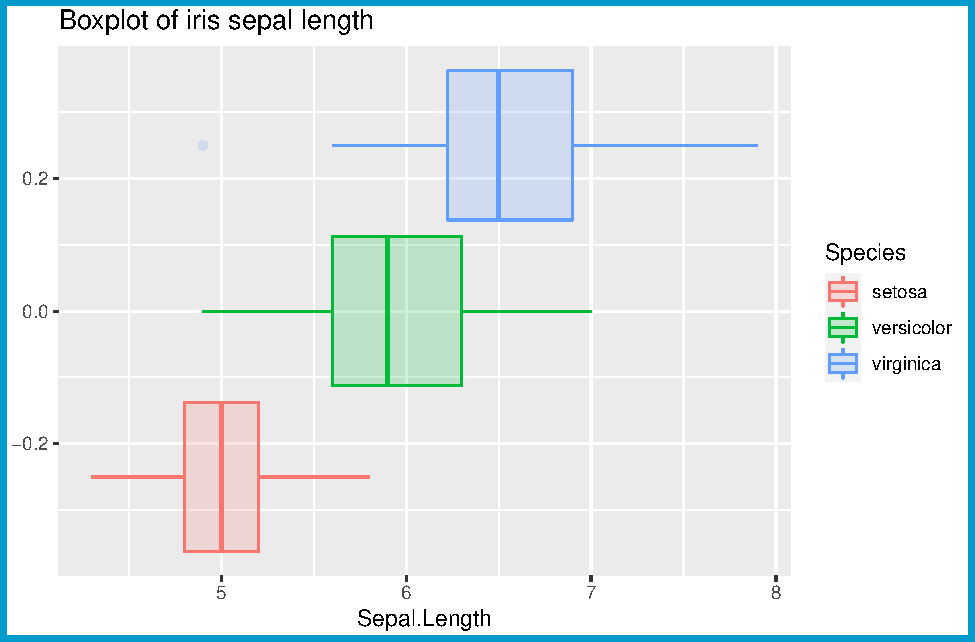
\includegraphics{test_1.pdf}
\end{figure}

\begin{figure}[h!]
\caption{This is another test.}
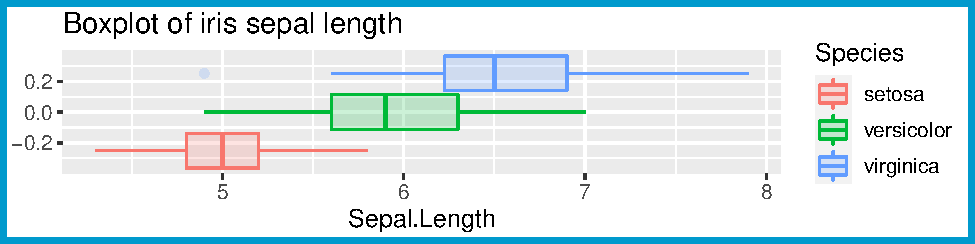
\includegraphics{test_2.pdf}
\end{figure}

\end{document}